\chapter{Hasil Eksperimen di Jalan}
\label{lamp:C}
\section{Topologi Star}
\subsection{Rectangle Window}
\begin{itemize}
\item Sensor1
\begin{figure}[H]
	\centering
	\includegraphics[scale=0.5]{PengujianEksperimental/StarRectangleRoad/11}
	\caption[Hasil Sensing Sensor1 dengan topologi star dan window {\it Rectangle} di Jalan]{Hasil Sensing Sensor1 dengan topologi star dan window {\it Rectangle} di Jalan} 
	\label{fig:hasilJalanStarRect11}
\end{figure}

\begin{figure}[H]
	\centering
	\includegraphics[scale=0.5]{PengujianEksperimental/StarRectangleRoad/1,1}
	\caption[Hasil Spectrogram Sensor1 dengan topologi star dan window {\it Rectangle} di Jalan]{Hasil Spectrogram Sensor1 dengan topologi star dan window {\it Rectangle} di Jalan} 
	\label{fig:hasilJalanStarRect1,1}
\end{figure}

\item Sensor2
\begin{figure}[H]
	\centering
	\includegraphics[scale=0.5]{PengujianEksperimental/StarRectangleRoad/21}
	\caption[Hasil Sensing Sensor2 dengan topologi star dan window {\it Rectangle} di Jalan]{Hasil Sensing Sensor2 dengan topologi star dan window {\it Rectangle} di Jalan} 
	\label{fig:hasilJalanStarRect21}
\end{figure}

\begin{figure}[H]
	\centering
	\includegraphics[scale=0.5]{PengujianEksperimental/StarRectangleRoad/2,1}
	\caption[Hasil Spectrogram Sensor2 dengan topologi star dan window {\it Rectangle} di Jalan]{Hasil Spectrogram Sensor2 dengan topologi star dan window {\it Rectangle} di Jalan} 
	\label{fig:hasilJalanStarRect2,1}
\end{figure}

\item Sensor3
\begin{figure}[H]
	\centering
	\includegraphics[scale=0.5]{PengujianEksperimental/StarRectangleRoad/31}
	\caption[Hasil Sensing Sensor3 dengan topologi star dan window {\it Rectangle} di Jalan]{Hasil Sensing Sensor3 dengan topologi star dan window {\it Rectangle} di Jalan} 
	\label{fig:hasilJalanStarRect31}
\end{figure}

\begin{figure}[H]
	\centering
	\includegraphics[scale=0.5]{PengujianEksperimental/StarRectangleRoad/3,1}
	\caption[Hasil Spectrogram Sensor3 dengan topologi star dan window {\it Rectangle} di Jalan]{Hasil Spectrogram Sensor3 dengan topologi star dan window {\it Rectangle} di Jalan} 
	\label{fig:hasilJalanStarRect3,1}
\end{figure}

\item Sensor4
\begin{figure}[H]
	\centering
	\includegraphics[scale=0.5]{PengujianEksperimental/StarRectangleRoad/41}
	\caption[Hasil Sensing Sensor4 dengan topologi star dan window {\it Rectangle} di Jalan]{Hasil Sensing Sensor4 dengan topologi star dan window {\it Rectangle} di Jalan} 
	\label{fig:hasilJalanStarRect41}
\end{figure}

\begin{figure}[H]
	\centering
	\includegraphics[scale=0.5]{PengujianEksperimental/StarRectangleRoad/4,1}
	\caption[Hasil Spectrogram Sensor4 dengan topologi star dan window {\it Rectangle} di Jalan]{Hasil Spectrogram Sensor4 dengan topologi star dan window {\it Rectangle} di Jalan} 
	\label{fig:hasilJalanStarRect4,1}
\end{figure}

\item Sensor5
\begin{figure}[H]
	\centering
	\includegraphics[scale=0.5]{PengujianEksperimental/StarRectangleRoad/51}
	\caption[Hasil Sensing Sensor5 dengan topologi star dan window {\it Rectangle} di Jalan]{Hasil Sensing Sensor5 dengan topologi star dan window {\it Rectangle} di Jalan} 
	\label{fig:hasilJalanStarRect51}
\end{figure}

\begin{figure}[H]
	\centering
	\includegraphics[scale=0.5]{PengujianEksperimental/StarRectangleRoad/5,1}
	\caption[Hasil Spectrogram Sensor5 dengan topologi star dan window {\it Rectangle} di Jalan]{Hasil Spectrogram Sensor5 dengan topologi star dan window {\it Rectangle} di Jalan} 
	\label{fig:hasilJalanStarRect5,1}
\end{figure}
\end{itemize}

\subsection{Hanning Window}
\begin{itemize}
\item Sensor1
\begin{figure}[H]
	\centering
	\includegraphics[scale=0.5]{PengujianEksperimental/StarHanningRoad/11}
	\caption[Hasil Sensing Sensor1 dengan topologi star dan window {\it Hanning} di Jalan]{Hasil Sensing Sensor1 dengan topologi star dan window {\it Hanning} di Jalan} 
	\label{fig:hasilJalanStarHann11}
\end{figure}

\begin{figure}[H]
	\centering
	\includegraphics[scale=0.5]{PengujianEksperimental/StarHanningRoad/1,1}
	\caption[Hasil Spectrogram Sensor1 dengan topologi star dan window {\it Hanning} di Jalan]{Hasil Spectrogram Sensor1 dengan topologi star dan window {\it Hanning} di Jalan} 
	\label{fig:hasilJalanStarHann1,1}
\end{figure}

\item Sensor2
\begin{figure}[H]
	\centering
	\includegraphics[scale=0.5]{PengujianEksperimental/StarHanningRoad/21}
	\caption[Hasil Sensing Sensor2 dengan topologi star dan window {\it Hanning} di Jalan]{Hasil Sensing Sensor2 dengan topologi star dan window {\it Hanning} di Jalan} 
	\label{fig:hasilJalanStarHann21}
\end{figure}

\begin{figure}[H]
	\centering
	\includegraphics[scale=0.5]{PengujianEksperimental/StarHanningRoad/2,1}
	\caption[Hasil Spectrogram Sensor2 dengan topologi star dan window {\it Hanning} di Jalan]{Hasil Spectrogram Sensor2 dengan topologi star dan window {\it Hanning} di Jalan} 
	\label{fig:hasilJalanStarHann2,1}
\end{figure}

\item Sensor3
\begin{figure}[H]
	\centering
	\includegraphics[scale=0.5]{PengujianEksperimental/StarHanningRoad/31}
	\caption[Hasil Sensing Sensor3 dengan topologi star dan window {\it Hanning} di Jalan]{Hasil Sensing Sensor3 dengan topologi star dan window {\it Hanning} di Jalan} 
	\label{fig:hasilJalanStarHann31}
\end{figure}

\begin{figure}[H]
	\centering
	\includegraphics[scale=0.5]{PengujianEksperimental/StarHanningRoad/3,1}
	\caption[Hasil Spectrogram Sensor3 dengan topologi star dan window {\it Hanning} di Jalan]{Hasil Spectrogram Sensor3 dengan topologi star dan window {\it Hanning} di Jalan} 
	\label{fig:hasilJalanStarHann3,1}
\end{figure}

\item Sensor4
\begin{figure}[H]
	\centering
	\includegraphics[scale=0.5]{PengujianEksperimental/StarHanningRoad/41}
	\caption[Hasil Sensing Sensor4 dengan topologi star dan window {\it Hanning} di Jalan]{Hasil Sensing Sensor4 dengan topologi star dan window {\it Hanning} di Jalan} 
	\label{fig:hasilJalanStarHann41}
\end{figure}

\begin{figure}[H]
	\centering
	\includegraphics[scale=0.5]{PengujianEksperimental/StarHanningRoad/4,1}
	\caption[Hasil Spectrogram Sensor4 dengan topologi star dan window {\it Hanning} di Jalan]{Hasil Spectrogram Sensor4 dengan topologi star dan window {\it Hanning} di Jalan} 
	\label{fig:hasilJalanStarHann4,1}
\end{figure}

\item Sensor5
\begin{figure}[H]
	\centering
	\includegraphics[scale=0.5]{PengujianEksperimental/StarHanningRoad/51}
	\caption[Hasil Sensing Sensor5 dengan topologi star dan window {\it Hanning} di Jalan]{Hasil Sensing Sensor5 dengan topologi star dan window {\it Hanning} di Jalan} 
	\label{fig:hasilJalanStarHann51}
\end{figure}

\begin{figure}[H]
	\centering
	\includegraphics[scale=0.5]{PengujianEksperimental/StarHanningRoad/5,1}
	\caption[Hasil Spectrogram Sensor5 dengan topologi star dan window {\it Hanning} di Jalan]{Hasil Spectrogram Sensor5 dengan topologi star dan window {\it Hanning} di Jalan} 
	\label{fig:hasilJalanStarHann5,1}
\end{figure}
\end{itemize}

\subsection{Hamming Window}
\begin{itemize}
\item Sensor1
\begin{figure}[H]
	\centering
	\includegraphics[scale=0.5]{PengujianEksperimental/StarHammingRoad/11}
	\caption[Hasil Sensing Sensor1 dengan topologi star dan window {\it Hamming} di Jalan]{Hasil Sensing Sensor1 dengan topologi star dan window {\it Hamming} di Jalan} 
	\label{fig:hasilJalanStarHamm11}
\end{figure}

\begin{figure}[H]
	\centering
	\includegraphics[scale=0.5]{PengujianEksperimental/StarHammingRoad/1,1}
	\caption[Hasil Spectrogram Sensor1 dengan topologi star dan window {\it Hamming} di Jalan]{Hasil Spectrogram Sensor1 dengan topologi star dan window {\it Hamming} di Jalan} 
	\label{fig:hasilJalanStarHamm1,1}
\end{figure}

\item Sensor2
\begin{figure}[H]
	\centering
	\includegraphics[scale=0.5]{PengujianEksperimental/StarHammingRoad/21}
	\caption[Hasil Sensing Sensor2 dengan topologi star dan window {\it Hamming} di Jalan]{Hasil Sensing Sensor2 dengan topologi star dan window {\it Hamming} di Jalan} 
	\label{fig:hasilJalanStarHamm21}
\end{figure}

\begin{figure}[H]
	\centering
	\includegraphics[scale=0.5]{PengujianEksperimental/StarHammingRoad/2,1}
	\caption[Hasil Spectrogram Sensor2 dengan topologi star dan window {\it Hamming} di Jalan]{Hasil Spectrogram Sensor2 dengan topologi star dan window {\it Hamming} di Jalan} 
	\label{fig:hasilJalanStarHamm2,1}
\end{figure}

\item Sensor3
\begin{figure}[H]
	\centering
	\includegraphics[scale=0.5]{PengujianEksperimental/StarHammingRoad/31}
	\caption[Hasil Sensing Sensor3 dengan topologi star dan window {\it Hamming} di Jalan]{Hasil Sensing Sensor3 dengan topologi star dan window {\it Hamming} di Jalan} 
	\label{fig:hasilJalanStarHamm31}
\end{figure}

\begin{figure}[H]
	\centering
	\includegraphics[scale=0.5]{PengujianEksperimental/StarHammingRoad/3,1}
	\caption[Hasil Spectrogram Sensor3 dengan topologi star dan window {\it Hamming} di Jalan]{Hasil Spectrogram Sensor3 dengan topologi star dan window {\it Hamming} di Jalan} 
	\label{fig:hasilJalanStarHamm3,1}
\end{figure}

\item Sensor4
\begin{figure}[H]
	\centering
	\includegraphics[scale=0.5]{PengujianEksperimental/StarHammingRoad/41}
	\caption[Hasil Sensing Sensor4 dengan topologi star dan window {\it Hamming} di Jalan]{Hasil Sensing Sensor4 dengan topologi star dan window {\it Hamming} di Jalan} 
	\label{fig:hasilJalanStarHamm41}
\end{figure}

\begin{figure}[H]
	\centering
	\includegraphics[scale=0.5]{PengujianEksperimental/StarHammingRoad/4,1}
	\caption[Hasil Spectrogram Sensor4 dengan topologi star dan window {\it Hamming} di Jalan]{Hasil Spectrogram Sensor4 dengan topologi star dan window {\it Hamming} di Jalan} 
	\label{fig:hasilJalanStarHamm4,1}
\end{figure}

\item Sensor5
\begin{figure}[H]
	\centering
	\includegraphics[scale=0.5]{PengujianEksperimental/StarHammingRoad/51}
	\caption[Hasil Sensing Sensor5 dengan topologi star dan window {\it Hamming} di Jalan]{Hasil Sensing Sensor5 dengan topologi star dan window {\it Hamming} di Jalan} 
	\label{fig:hasilJalanStarHamm51}
\end{figure}

\begin{figure}[H]
	\centering
	\includegraphics[scale=0.5]{PengujianEksperimental/StarHammingRoad/5,1}
	\caption[Hasil Spectrogram Sensor5 dengan topologi star dan window {\it Hamming} di Jalan]{Hasil Spectrogram Sensor5 dengan topologi star dan window {\it Hamming} di Jalan} 
	\label{fig:hasilJalanStarHamm5,1}
\end{figure}
\end{itemize}

\section{Topologi Tree}
\subsection{Rectangle Window}
\begin{itemize}
\item Sensor1
\begin{figure}[H]
	\centering
	\includegraphics[scale=0.5]{PengujianEksperimental/TreeRectangleRoad/11}
	\caption[Hasil Sensing Sensor1 dengan topologi tree dan window {\it Rectangle} di Jalan]{Hasil Sensing Sensor1 dengan topologi tree dan window {\it Rectangle} di Jalan} 
	\label{fig:hasilJalanTreeRect11}
\end{figure}

\begin{figure}[H]
	\centering
	\includegraphics[scale=0.5]{PengujianEksperimental/TreeRectangleRoad/1,1}
	\caption[Hasil Spectrogram Sensor1 dengan topologi tree dan window {\it Rectangle} di Jalan]{Hasil Spectrogram Sensor1 dengan topologi tree dan window {\it Rectangle} di Jalan} 
	\label{fig:hasilJalanTreeRect1,1}
\end{figure}

\item Sensor2
\begin{figure}[H]
	\centering
	\includegraphics[scale=0.5]{PengujianEksperimental/TreeRectangleRoad/21}
	\caption[Hasil Sensing Sensor2 dengan topologi tree dan window {\it Rectangle} di Jalan]{Hasil Sensing Sensor2 dengan topologi tree dan window {\it Rectangle} di Jalan} 
	\label{fig:hasilJalanTreeRect21}
\end{figure}

\begin{figure}[H]
	\centering
	\includegraphics[scale=0.5]{PengujianEksperimental/TreeRectangleRoad/2,1}
	\caption[Hasil Spectrogram Sensor2 dengan topologi tree dan window {\it Rectangle} di Jalan]{Hasil Spectrogram Sensor2 dengan topologi tree dan window {\it Rectangle} di Jalan} 
	\label{fig:hasilJalanTreeRect2,1}
\end{figure}

\item Sensor3
\begin{figure}[H]
	\centering
	\includegraphics[scale=0.5]{PengujianEksperimental/TreeRectangleRoad/31}
	\caption[Hasil Sensing Sensor3 dengan topologi tree dan window {\it Rectangle} di Jalan]{Hasil Sensing Sensor3 dengan topologi tree dan window {\it Rectangle} di Jalan} 
	\label{fig:hasilJalanTreeRect31}
\end{figure}

\begin{figure}[H]
	\centering
	\includegraphics[scale=0.5]{PengujianEksperimental/TreeRectangleRoad/3,1}
	\caption[Hasil Spectrogram Sensor3 dengan topologi tree dan window {\it Rectangle} di Jalan]{Hasil Spectrogram Sensor3 dengan topologi tree dan window {\it Rectangle} di Jalan} 
	\label{fig:hasilJalanTreeRect3,1}
\end{figure}

\item Sensor4
\begin{figure}[H]
	\centering
	\includegraphics[scale=0.5]{PengujianEksperimental/TreeRectangleRoad/41}
	\caption[Hasil Sensing Sensor4 dengan topologi tree dan window {\it Rectangle} di Jalan]{Hasil Sensing Sensor4 dengan topologi tree dan window {\it Rectangle} di Jalan} 
	\label{fig:hasilJalanTreeRect41}
\end{figure}

\begin{figure}[H]
	\centering
	\includegraphics[scale=0.5]{PengujianEksperimental/TreeRectangleRoad/4,1}
	\caption[Hasil Spectrogram Sensor4 dengan topologi tree dan window {\it Rectangle} di Jalan]{Hasil Spectrogram Sensor4 dengan topologi tree dan window {\it Rectangle} di Jalan} 
	\label{fig:hasilJalanTreeRect4,1}
\end{figure}

\item Sensor5
\begin{figure}[H]
	\centering
	\includegraphics[scale=0.5]{PengujianEksperimental/TreeRectangleRoad/51}
	\caption[Hasil Sensing Sensor5 dengan topologi tree dan window {\it Rectangle} di Jalan]{Hasil Sensing Sensor5 dengan topologi tree dan window {\it Rectangle} di Jalan} 
	\label{fig:hasilJalanTreeRect51}
\end{figure}

\begin{figure}[H]
	\centering
	\includegraphics[scale=0.5]{PengujianEksperimental/TreeRectangleRoad/5,1}
	\caption[Hasil Spectrogram Sensor5 dengan topologi tree dan window {\it Rectangle} di Jalan]{Hasil Spectrogram Sensor5 dengan topologi tree dan window {\it Rectangle} di Jalan} 
	\label{fig:hasilJalanTreeRect5,1}
\end{figure}
\end{itemize}

\subsection{Hanning Window}
\begin{itemize}
\item Sensor1
\begin{figure}[H]
	\centering
	\includegraphics[scale=0.5]{PengujianEksperimental/TreeHanningRoad/11}
	\caption[Hasil Sensing Sensor1 dengan topologi tree dan window {\it Hanning} di Jalan]{Hasil Sensing Sensor1 dengan topologi tree dan window {\it Hanning} di Jalan} 
	\label{fig:hasilJalanTreeHann11}
\end{figure}

\begin{figure}[H]
	\centering
	\includegraphics[scale=0.5]{PengujianEksperimental/TreeHanningRoad/1,1}
	\caption[Hasil Spectrogram Sensor1 dengan topologi tree dan window {\it Hanning} di Jalan]{Hasil Spectrogram Sensor1 dengan topologi tree dan window {\it Hanning} di Jalan} 
	\label{fig:hasilJalanTreeHann1,1}
\end{figure}

\item Sensor2
\begin{figure}[H]
	\centering
	\includegraphics[scale=0.5]{PengujianEksperimental/TreeHanningRoad/21}
	\caption[Hasil Sensing Sensor2 dengan topologi tree dan window {\it Hanning} di Jalan]{Hasil Sensing Sensor2 dengan topologi tree dan window {\it Hanning} di Jalan} 
	\label{fig:hasilJalanTreeHann21}
\end{figure}

\begin{figure}[H]
	\centering
	\includegraphics[scale=0.5]{PengujianEksperimental/TreeHanningRoad/2,1}
	\caption[Hasil Spectrogram Sensor2 dengan topologi tree dan window {\it Hanning} di Jalan]{Hasil Spectrogram Sensor2 dengan topologi tree dan window {\it Hanning} di Jalan} 
	\label{fig:hasilJalanTreeHann2,1}
\end{figure}

\item Sensor3
\begin{figure}[H]
	\centering
	\includegraphics[scale=0.5]{PengujianEksperimental/TreeHanningRoad/31}
	\caption[Hasil Sensing Sensor3 dengan topologi tree dan window {\it Hanning} di Jalan]{Hasil Sensing Sensor3 dengan topologi tree dan window {\it Hanning} di Jalan} 
	\label{fig:hasilJalanTreeHann31}
\end{figure}

\begin{figure}[H]
	\centering
	\includegraphics[scale=0.5]{PengujianEksperimental/TreeHanningRoad/3,1}
	\caption[Hasil Spectrogram Sensor3 dengan topologi tree dan window {\it Hanning} di Jalan]{Hasil Spectrogram Sensor3 dengan topologi tree dan window {\it Hanning} di Jalan} 
	\label{fig:hasilJalanTreeHann3,1}
\end{figure}

\item Sensor4
\begin{figure}[H]
	\centering
	\includegraphics[scale=0.5]{PengujianEksperimental/TreeHanningRoad/41}
	\caption[Hasil Sensing Sensor4 dengan topologi tree dan window {\it Hanning} di Jalan]{Hasil Sensing Sensor4 dengan topologi tree dan window {\it Hanning} di Jalan} 
	\label{fig:hasilJalanTreeHann41}
\end{figure}

\begin{figure}[H]
	\centering
	\includegraphics[scale=0.5]{PengujianEksperimental/TreeHanningRoad/4,1}
	\caption[Hasil Spectrogram Sensor4 dengan topologi tree dan window {\it Hanning} di Jalan]{Hasil Spectrogram Sensor4 dengan topologi tree dan window {\it Hanning} di Jalan} 
	\label{fig:hasilJalanTreeHann4,1}
\end{figure}

\item Sensor5
\begin{figure}[H]
	\centering
	\includegraphics[scale=0.5]{PengujianEksperimental/TreeHanningRoad/51}
	\caption[Hasil Sensing Sensor5 dengan topologi tree dan window {\it Hanning} di Jalan]{Hasil Sensing Sensor5 dengan topologi tree dan window {\it Hanning} di Jalan} 
	\label{fig:hasilJalanTreeHann51}
\end{figure}

\begin{figure}[H]
	\centering
	\includegraphics[scale=0.5]{PengujianEksperimental/TreeHanningRoad/5,1}
	\caption[Hasil Spectrogram Sensor5 dengan topologi tree dan window {\it Hanning} di Jalan]{Hasil Spectrogram Sensor5 dengan topologi tree dan window {\it Hanning} di Jalan} 
	\label{fig:hasilJalanTreeHann5,1}
\end{figure}
\end{itemize}

\subsection{Hamming Window}
\begin{itemize}
\item Sensor1
\begin{figure}[H]
	\centering
	\includegraphics[scale=0.5]{PengujianEksperimental/TreeHammingRoad/11}
	\caption[Hasil Sensing Sensor1 dengan topologi tree dan window {\it Hamming} di Jalan]{Hasil Sensing Sensor1 dengan topologi tree dan window {\it Hamming} di Jalan} 
	\label{fig:hasilJalanTreeHamm11}
\end{figure}

\begin{figure}[H]
	\centering
	\includegraphics[scale=0.5]{PengujianEksperimental/TreeHammingRoad/1,1}
	\caption[Hasil Spectrogram Sensor1 dengan topologi tree dan window {\it Hamming} di Jalan]{Hasil Spectrogram Sensor1 dengan topologi tree dan window {\it Hamming} di Jalan} 
	\label{fig:hasilJalanTreeHamm1,1}
\end{figure}

\item Sensor2
\begin{figure}[H]
	\centering
	\includegraphics[scale=0.5]{PengujianEksperimental/TreeHammingRoad/21}
	\caption[Hasil Sensing Sensor2 dengan topologi tree dan window {\it Hamming} di Jalan]{Hasil Sensing Sensor2 dengan topologi tree dan window {\it Hamming} di Jalan} 
	\label{fig:hasilJalanTreeHamm21}
\end{figure}

\begin{figure}[H]
	\centering
	\includegraphics[scale=0.5]{PengujianEksperimental/TreeHammingRoad/2,1}
	\caption[Hasil Spectrogram Sensor2 dengan topologi tree dan window {\it Hamming} di Jalan]{Hasil Spectrogram Sensor2 dengan topologi tree dan window {\it Hamming} di Jalan} 
	\label{fig:hasilJalanTreeHamm2,1}
\end{figure}

\item Sensor3
\begin{figure}[H]
	\centering
	\includegraphics[scale=0.5]{PengujianEksperimental/TreeHammingRoad/31}
	\caption[Hasil Sensing Sensor3 dengan topologi tree dan window {\it Hamming} di Jalan]{Hasil Sensing Sensor3 dengan topologi tree dan window {\it Hamming} di Jalan} 
	\label{fig:hasilJalanTreeHamm31}
\end{figure}

\begin{figure}[H]
	\centering
	\includegraphics[scale=0.5]{PengujianEksperimental/TreeHammingRoad/3,1}
	\caption[Hasil Spectrogram Sensor3 dengan topologi tree dan window {\it Hamming} di Jalan]{Hasil Spectrogram Sensor3 dengan topologi tree dan window {\it Hamming} di Jalan} 
	\label{fig:hasilJalanTreeHamm3,1}
\end{figure}

\item Sensor4
\begin{figure}[H]
	\centering
	\includegraphics[scale=0.5]{PengujianEksperimental/TreeHammingRoad/41}
	\caption[Hasil Sensing Sensor4 dengan topologi tree dan window {\it Hamming} di Jalan]{Hasil Sensing Sensor4 dengan topologi tree dan window {\it Hamming} di Jalan} 
	\label{fig:hasilJalanTreeHamm41}
\end{figure}

\begin{figure}[H]
	\centering
	\includegraphics[scale=0.5]{PengujianEksperimental/TreeHammingRoad/4,1}
	\caption[Hasil Spectrogram Sensor4 dengan topologi tree dan window {\it Hamming} di Jalan]{Hasil Spectrogram Sensor4 dengan topologi tree dan window {\it Hamming} di Jalan} 
	\label{fig:hasilJalanTreeHamm4,1}
\end{figure}

\item Sensor5
\begin{figure}[H]
	\centering
	\includegraphics[scale=0.5]{PengujianEksperimental/TreeHammingRoad/51}
	\caption[Hasil Sensing Sensor5 dengan topologi tree dan window {\it Hamming} di Jalan]{Hasil Sensing Sensor5 dengan topologi tree dan window {\it Hamming} di Jalan} 
	\label{fig:hasilJalanTreeHamm51}
\end{figure}

\begin{figure}[H]
	\centering
	\includegraphics[scale=0.5]{PengujianEksperimental/TreeHammingRoad/5,1}
	\caption[Hasil Spectrogram Sensor5 dengan topologi tree dan window {\it Hamming} di Jalan]{Hasil Spectrogram Sensor5 dengan topologi tree dan window {\it Hamming} di Jalan} 
	\label{fig:hasilJalanTreeHamm5,1}
\end{figure}
\end{itemize}